\pdfminorversion=6
\documentclass[
	usepdftitle=false,
% 	handout,
% 	notes,
% 	fleqn,
	hyperref={
		pdfauthor={Stephan Waldchen},
		pdftitle={BIOQIC-Day-MRE-Denoising},
		pdfsubject={Workshop},
		pdfcreator={LaTeX},
	}
]{beamer}
\usepackage[utf8]{inputenc}
\usepackage{default}


\newcommand{\kl}[1]{\left( #1 \right)}
\newcommand{\ekl}[1]{\left[ #1 \right]}
\newcommand{\skl}[1]{\left\{ #1 \right\}}
\newcommand{\bkl}[1]{\left| #1 \right|}

\newcommand{\tdf}[2]{\frac{\text{d#1}}{\text{d} #2}}

\newcommand{\xb}[1]{\mathbf{x}}


%Information to be included in the title page:
% \title{Anisotropic MRE}
% \author{Stephan W\"{a}ldchen}
% \institute{BIOQIC - a cooperation between TU BErlin and Charite}
% \date{\today}
%  
%  

% ------------- Packages

% \usepackage{default}

%%% Doc: http://mirror.informatik.uni-mannheim.de/pub/mirrors/tex-archive/macros/latex/contrib/xargs/xargs.pdf
% More than one optional argument
\usepackage{xargs}

%%%
% IfThenElse
\usepackage{ifthen}

%%% Doc: ftp://ftp.mpi-sb.mpg.de/pub/tex/mirror/ftp.dante.de/pub/tex/macros/latex/contrib/etoolbox/etoolbox.pdf
% Programming in LaTeX
\usepackage{etoolbox}

%%% Doc: ftp://tug.ctan.org/pub/tex-archive/macros/latex/required/babel/babel.pdf
% Language setting
\usepackage[
%	german,
% 	ngerman,
	english,
%	french,
]{babel}

%%% Doc: ftp://tug.ctan.org/pub/tex-archive/macros/latex/required/graphics/grfguide.pdf
% Graphics
\usepackage[%
	%final,
	%draft % do not include images (faster)
]{graphicx}

\def\Put(#1,#2)#3{\leavevmode\makebox(0,0){\put(#1,#2){#3}}}

\usepackage{array}

\usepackage{wrapfig}

% \usepackage{memh­fixc}
% \usepackage{memoir}

\usepackage{relsize}

\usepackage{mdframed}

% \usepackage{enumitem}

%%%
% This package is used to create two-sided presentations with notes
\usepackage{pgfpages}

\usepackage{tikz}
\usetikzlibrary{arrows,shapes,calc}
\newcommand{\tikzmark}[2]{\tikz[overlay,remember picture] \node[minimum width=1.5em] (#1) {#2};}
\newcommand{\tikzcoord}[1]{\tikz[overlay,remember picture] \coordinate (#1);}
\makeatletter
\protected\def\tikz@nonactivecolon{\ifmmode\mathrel{\mathop\ordinarycolon}\else:\fi} 
\makeatother

\newcommand*\circled[1]{\tikz[baseline=(char.base)]{
            \node[shape=circle,draw,inner sep=2pt] (char) {#1};}}


% Put text somewhere on the slide
% \def\Put(#1,#2)#3{\leavevmode\makebox(0,0){\put(#1,#2){#3}}}
\usepackage{textpos}

%%% Doc: ftp://tug.ctan.org/pub/tex-archive/macros/latex/contrib/mh/doc/mathtools.pdf
% Erweitert amsmath und behebt einige Bugs
\usepackage[fixamsmath,disallowspaces]{mathtools}
% Formelnummern nur anzeigen, wenn auch eine Referenz existiert
\mathtoolsset{showonlyrefs}
\mathtoolsset{centercolon=true}
% \usepackage{autonum}

\usepackage{mathrsfs}

\usepackage{bm}

\usepackage{dsfont}

\usepackage{wasysym} % Smilies

% ------------- Definitions

%%% Programming
% Falls #2 definiert/nichtleer ist, so schreibe #3, sonst #1
\newcommand{\ifargdef}[3][{}]{\ifthenelse{\equal{#2}{}}{#1}{#3}}

%%% Colors
\definecolor{red}{rgb}{1,0,0}
\definecolor{blue}{rgb}{0,0,1}
\definecolor{green}{rgb}{0.2,0.6,0.15}
\definecolor{darkgreen}{rgb}{0,0.5,0}
\definecolor{lightblue}{rgb}{0,0.5,1}
\definecolor{white}{rgb}{1,1,1}
\definecolor{bluegreen}{rgb}{0,0.5,0.5}
\definecolor{violet}{rgb}{0.5,0,0.5}
\definecolor{ZurichBlue}{rgb}{.35,.35,.73}
\definecolor{TUred}{rgb}{0.7,0,0}
% \definecolor{red}{rgb}{1,0,0}
% \definecolor{blue}{rgb}{0,0,1}
% \definecolor{green}{rgb}{0.2,0.6,0.15}
% \definecolor{darkgreen}{rgb}{0,0.5,0}
% \definecolor{lightblue}{rgb}{0,0.5,1}
% %\definecolor{white}{rgb}{0,0,0}
% \definecolor{bluegreen}{rgb}{0,0.5,0.5}
% \definecolor{violet}{rgb}{0.5,0,0.5}
% \definecolor{ZurichBlue}{rgb}{.35,.35,.73}

\setbeamercolor{highlightbox}{fg=black,bg=ZurichBlue}

% no frame counting in appendix, use together with 'noframenumbering' as frame option
\makeatletter
\preto{\appendix}{%
  \patchcmd{\beamer@continueautobreak}{\refstepcounter{framenumber}}{}{}{}}
\makeatother

% Keep the frame title, if there is a framebreak
\setbeamertemplate{frametitle continuation}{}
% Break frame within a theorem
\newcommand*{\theorembreak}{\usebeamertemplate{theorem end}\framebreak\usebeamertemplate{theorem begin}}
% Definitions highlighting
\newcommand<>{\define}[1]{{\color#2{green} #1}}
\newcommand<>{\alertemph}[1]{{\color#2{red} #1}}

\newcommand{\citeref}[1]{{\tiny{\color{gray}#1}}}

\newtheorem{algorithm}{Algorithm}
\newtheorem{proposition}{Proposition}


% ------------- Settings

\mode<presentation>{
	\usetheme{Boadilla}
% 	\useoutertheme{infolines}
% 	\useinnertheme{rounded}
	\usecolortheme{beaver}
	\setbeamercovered{transparent}
	
% Make the default 'red' of beaver darker
	\definecolor{darkred}{rgb}{.65,0,0}
	\setbeamercolor{structure}{fg=ZurichBlue}
	
	\setbeamercolor{block title}{use=structure,fg=white,bg=darkred!80!white}
	\setbeamercolor{block body}{use=structure,fg=black,bg=gray!20!white}
	
	
	\setbeamercolor{frametitle}{bg=gray!20!white}
	
	% Frame title with logo in the right corner
	\setbeamertemplate{frametitle}
	{
		\nointerlineskip
		\begin{beamercolorbox}[sep=0.3cm,wd=\paperwidth]{frametitle}
			\vbox{}\vskip-1ex%
			\strut\insertframetitle\strut \hfill \mylogo
			\vskip-1.5ex%
		\end{beamercolorbox}
	}

% 	\setbeamertemplate{footline}[default]
% 	\setbeameroption{show notes on second screen}
% 	\setbeameroption{show notes}
	\setbeamercovered{invisible}
}

\beamertemplatenavigationsymbolsempty

\makeatletter
% add a macro that saves its argument
\newcommand{\footlineextra}[1]{\gdef\insertfootlineextra{#1}}
\newbox\footlineextrabox

% add a beamer template that sets the saved argument in a box.
% The * means that the beamer font and color "footline extra" are automatically added. 
\defbeamertemplate*{footline extra}{default}{
    \begin{beamercolorbox}[ht=2.25ex,dp=1ex,leftskip=\Gm@lmargin]{footline extra}
    \insertfootlineextra
    %\par\vspace{2.5pt}
    \end{beamercolorbox}
}

\addtobeamertemplate{footline}{%
    % set the box with the extra footline material but make it add no vertical space
    \setbox\footlineextrabox=\vbox{\usebeamertemplate*{footline extra}}
    \vskip -\ht\footlineextrabox
    \vskip -\dp\footlineextrabox
    \box\footlineextrabox%
}
{}

% patch \begin{frame} to reset the footline extra material
\let\beamer@original@frame=\frame
\def\frame{\gdef\insertfootlineextra{}\beamer@original@frame}
\footlineextra{}
\makeatother

\newcommand<>{\uncoverubrace}[2]{%
  \onslide#3 \underbrace{ \onslide<1->%
  #1%
  \onslide#3 }_{#2} \onslide<1->%
}

\setbeamertemplate{itemize items}[triangle]

\begin{document}

\title[Superimposed Sensor Measurements]{MRE Reconstruction: \\ Inverting the wave equation}
%%% Speaker
\author[Genzel \& Jung (TU Berlin)]{Stephan W\"{a}ldchen}

\institute[]{{}\\[-4ex](Technische Universität Berlin)}
%\\[2ex]
%{\footnotesize joint with}\\[2ex]
%{\normalsize Martin Genzel (Technische Universit\"at Berlin)}
%}
%%% date and place
\date[SPARS 2017]{BIOQIC Day 2017\\[.25em] Berlin (Germany) \\[.25em] \today \\[1ex]}
%%% Title logo
\titlegraphic{
\includegraphics[height=.9cm]{Images/AFG.png}\hspace{1cm}
\includegraphics[height=.9cm]{Images/BIOQIC-Logo.png}\hspace{1cm}\includegraphics[height=.9cm]{Images/TU_logo.pdf}}
%%% Talk logo
% \logo{\includegraphics[width=0.7cm,height=0.55cm]{Images/TU_logo.pdf}}
\newcommand{\mylogo}{\includegraphics[height=0.55cm]{Images/TU_logo.pdf}}

%%% Title frame
\begin{frame}[plain]
	\titlepage
\end{frame}

% \begin{frame}{Collaborators/Funding}

% \structure{Main Collaborator:}

% \begin{center}
% %\includegraphics[width=2.7cm]{Images/jung.jpeg}
% 
% Peter Jung \\[.5em] \smaller (Communications and Information Theory Group @ TU Berlin)
% \end{center}
% 
% \vspace{.5\baselineskip}
% 
% % \structure{Funding:}
% \begin{center}
% %\includegraphics[height=1.5cm]{Images/logo_ecmath.png} \qquad \includegraphics[height=1.5cm]{Images/dedale.png} \qquad \includegraphics[height=1cm]{Images/dfg_logo.jpeg}
% \end{center}
% 
% \end{frame}

\begin{frame}[noframenumbering]{Outline of This Talk}
	\tableofcontents
\end{frame}


\section{Why we need MRE}

% 
% \frame{\titlepage}

\begin{frame}[t]{Why do we need MRE?}

% \vspace{-\baselineskip}
% \begin{center}
% 	\define{Environmental monitoring problems} are of great \\ importance in many practical applications.
% \end{center}

% \vspace{.5\baselineskip}

\begin{columns}[T]
\column{.4\textwidth}
  \begin{itemize}
    \item<2-> diseased tissue changes mechanical
    \item<3-> low tech: palpation
    \item<4-> higher tech: ultrasound
    \item<5-> highest tech: MRE
    \item<6-> for deep tissue and brains, but non-invasive
  \end{itemize}
\column{.6\textwidth}

 	\vspace{-0.5cm}
	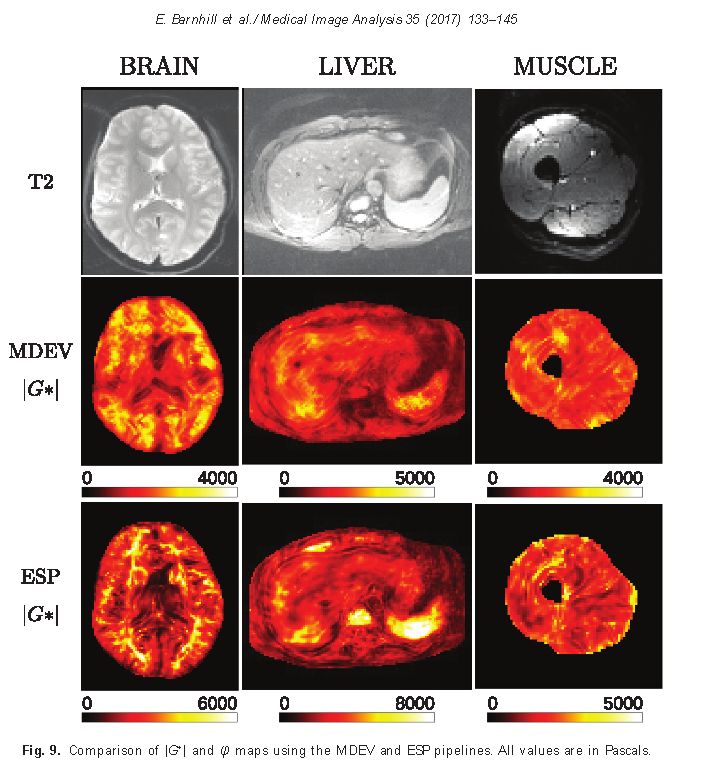
\includegraphics[width=\textwidth]{Images/Elasto-Tissue.pdf}

\end{columns}

\end{frame}



\begin{frame}{How does the measuring process work?}

\begin{figure}
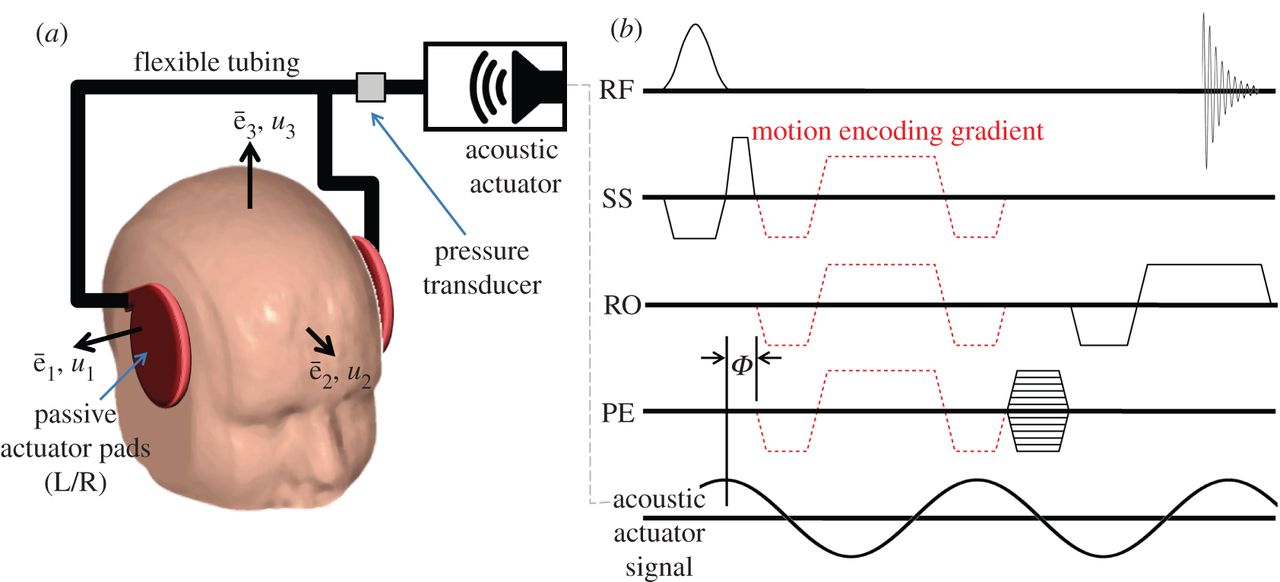
\includegraphics[width=0.9\textwidth]{Images/experiment.jpg}
\centering\end{figure}

\begin{itemize}
 \item<2-> 3 spatial directions $\times$ 8 time steps $\times$ 3 frequencies
 \item<3-> 72 times longer per pixel than MRI 
\end{itemize}

\end{frame}

\section{Data Reconstruction and current Problems}

\begin{frame}{How does the tissue movement relate to stiffness?}


\begin{itemize}
 \item<2-> Navier-Lam\'{e} equation:
 \begin{equation}
 \sum_ j \partial_j \kl{ \mu \kl{ \partial_j u_i + \partial_i u_j}} + \partial_i \kl{\lambda \partial_j u_j} = \rho \ddot{u}_i
\end{equation}
\item<3-> time harmonic and small bulk wave
 \begin{equation}
 \nabla(\bm{\mu}  \cdot \epsilon) = -\rho \omega^2 \mathbf{u} \quad \text{with} \quad \epsilon_{ij} = \partial_j u_i + \partial_i u_j
\end{equation}
 \item<4-> discretize the equation
 \begin{equation}
 \ekl{\nabla\cdot\epsilon + \epsilon\nabla} \bm{\mu} = -\rho \omega^2 \mathbf{u}
\end{equation}
 \item<5-> matrix inversion relies on correct knowledge of $\mathbf{u}^{'}$, and $\mathbf{u}^{''}$\\
 $\rightarrow$ noise can completely screw up the derivatives
\end{itemize}

\end{frame}


\begin{frame}{Noisy displacement field}

\begin{figure}
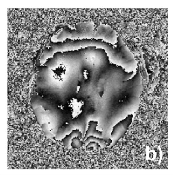
\includegraphics[width=0.5\textwidth]{Images/noisyBrain.png}
\caption{b) The human brain}
\centering\end{figure}

\end{frame}


\begin{frame}{Wavelet Denoising}

\begin{itemize}
 \item<2-> $\mathbf{u}(\mathbf{x},t)$ is piece-wise (very) smooth $\rightarrow$ sparse in wavelet domain
 \item<4-> in 2d: anisotropic structure $\rightarrow$ shearlets
\end{itemize}

\only<1-2>{
\vspace{5.1cm}
}

\only<3-4>{
\visible<3->{
\begin{figure}
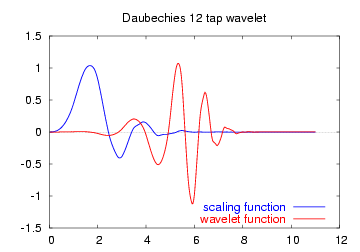
\includegraphics[width=0.5\textwidth]{Images/Daubechies.png}
\centering\end{figure}
}
}

\only<5>{
\vspace{0.95cm}
\begin{figure}
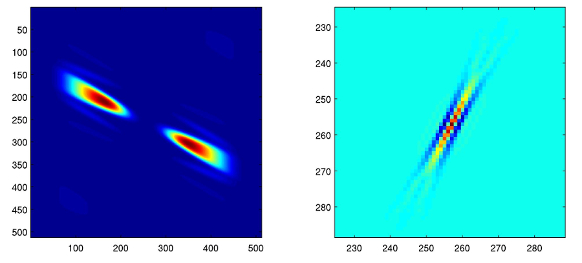
\includegraphics[width=0.6\textwidth]{Images/shearlet.jpeg}
\centering\end{figure}
}

\only<6->{
\vspace{1cm}
\begin{block}{Wavelet Denoising:}
 \begin{align}
  u^* &= \underset{u}{\text{argmin}}~\nkl{u_{\text{meas}} - u}^2_2 + \lambda \nkl{W u}_0 \\
      &= W^{\dagger} H\kl{W u_{\text{meas}}; \lambda}
 \end{align}
\end{block}
\vspace{1cm}
}


\end{frame}


% \begin{frame}		\frametitle{Data reconstruction}
% 
% 
% \begin{align}
%  \mathbf{u} &= \mathbf{u}(\xb,t) \\
%  \mu &=
% \end{align}
% 
% 
% 
% \begin{equation}
%  A\mathbf{\mu} = \mathbf{b}
% \end{equation}
% 
% 
% \end{frame}
% 
% \begin{frame}{Underdetermined System}
% 
% 
% \begin{itemize}
%  \item differential equation --> inverse problem
%  \item Problem underdetermined, we need boundary values
%  \item Problem: some regions are close to nodes --> no movement
%  \item Solution: Multi frequency inversion
%  \item Problem: Need to reconstruct the derivatives
%  \item motion encoding gradient
%  \item MRI measurement in 3 spatial directions and 8 time steps
% \end{itemize}
% 
% \begin{itemize}
%  \item MRI measurement in 3 spatial directions and 8 time steps and 3 frequencies --> 72 times MRI overhead
%  \item --> reduced resolution
% \end{itemize}
% 
% \begin{itemize}
% 
%  \item Problem: Need to reconstruct the derivatives
%  \item slight noise can lead to totally wrong derivatives --> inversion is useless
%  \item MRI measurement in 3 spatial directions and 8 time steps
% \end{itemize}
% 
% \end{frame}
% 
% \section{Denoising Techniques}


\begin{frame}
 
 \begin{figure}
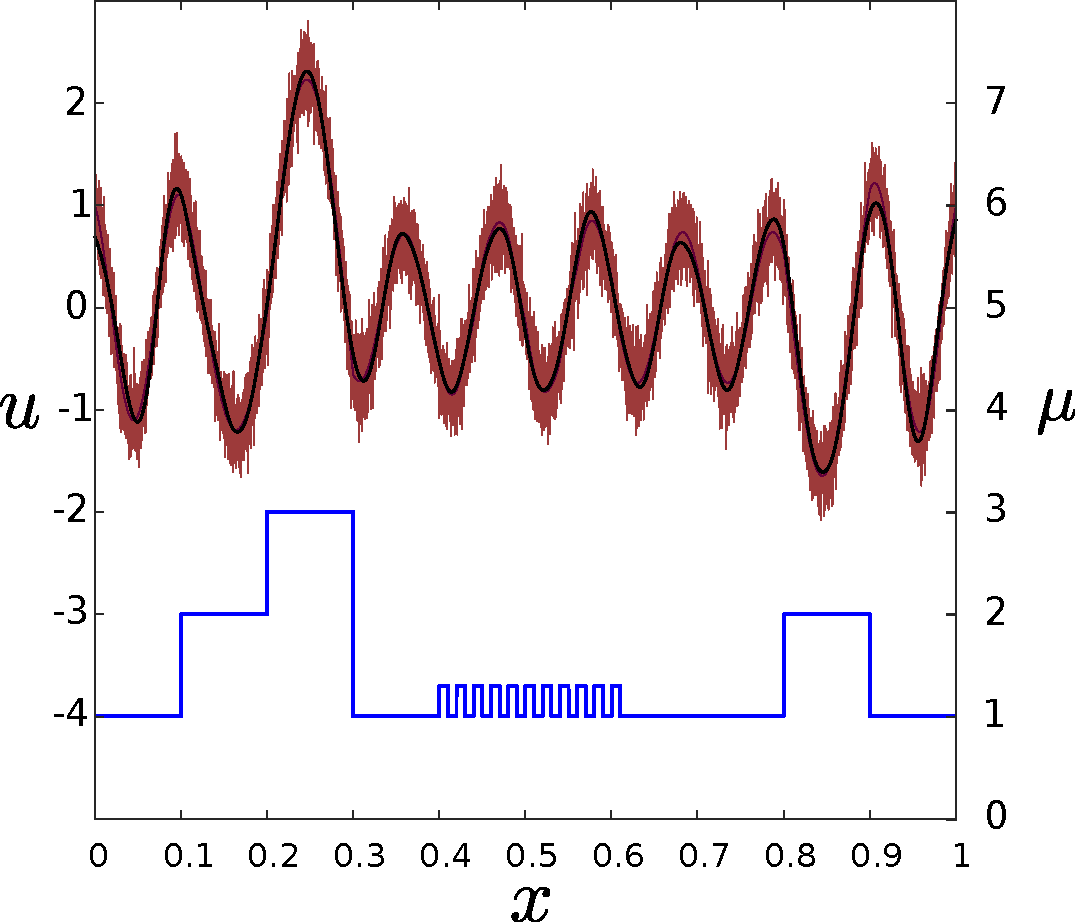
\includegraphics[width=0.7\textwidth]{Images/waveDenoising.pdf}
\centering
\caption{Shear parameter, displacement and noise in 1d}
\end{figure}
\end{frame}

\begin{frame}
 \begin{figure}
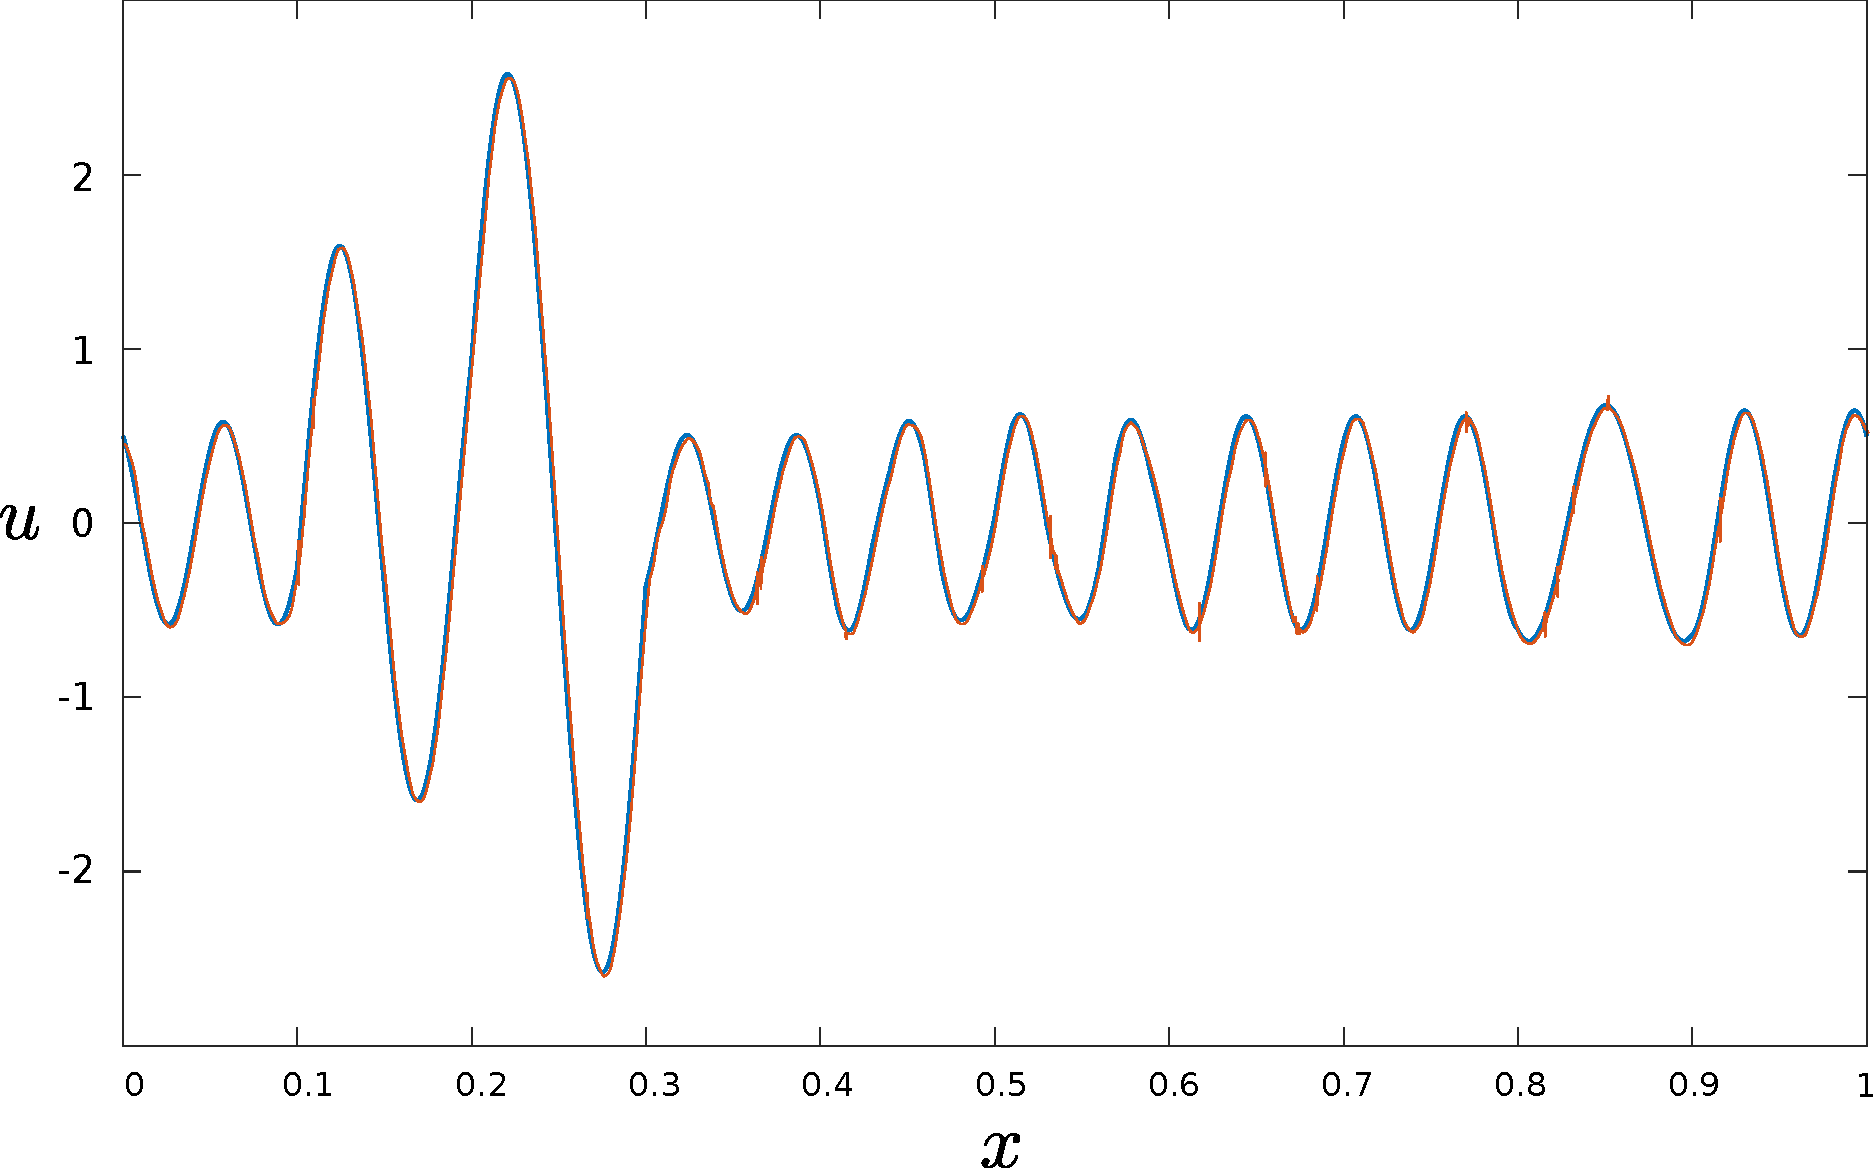
\includegraphics[width=0.8\textwidth]{Images/littleSpikes.pdf}
\caption{Reconstructed with Daubeshies10-wavelets and threshold of $0.01*\max_i(u_i)$}
\centering
\end{figure}
\end{frame}

\begin{frame}
 \begin{figure}
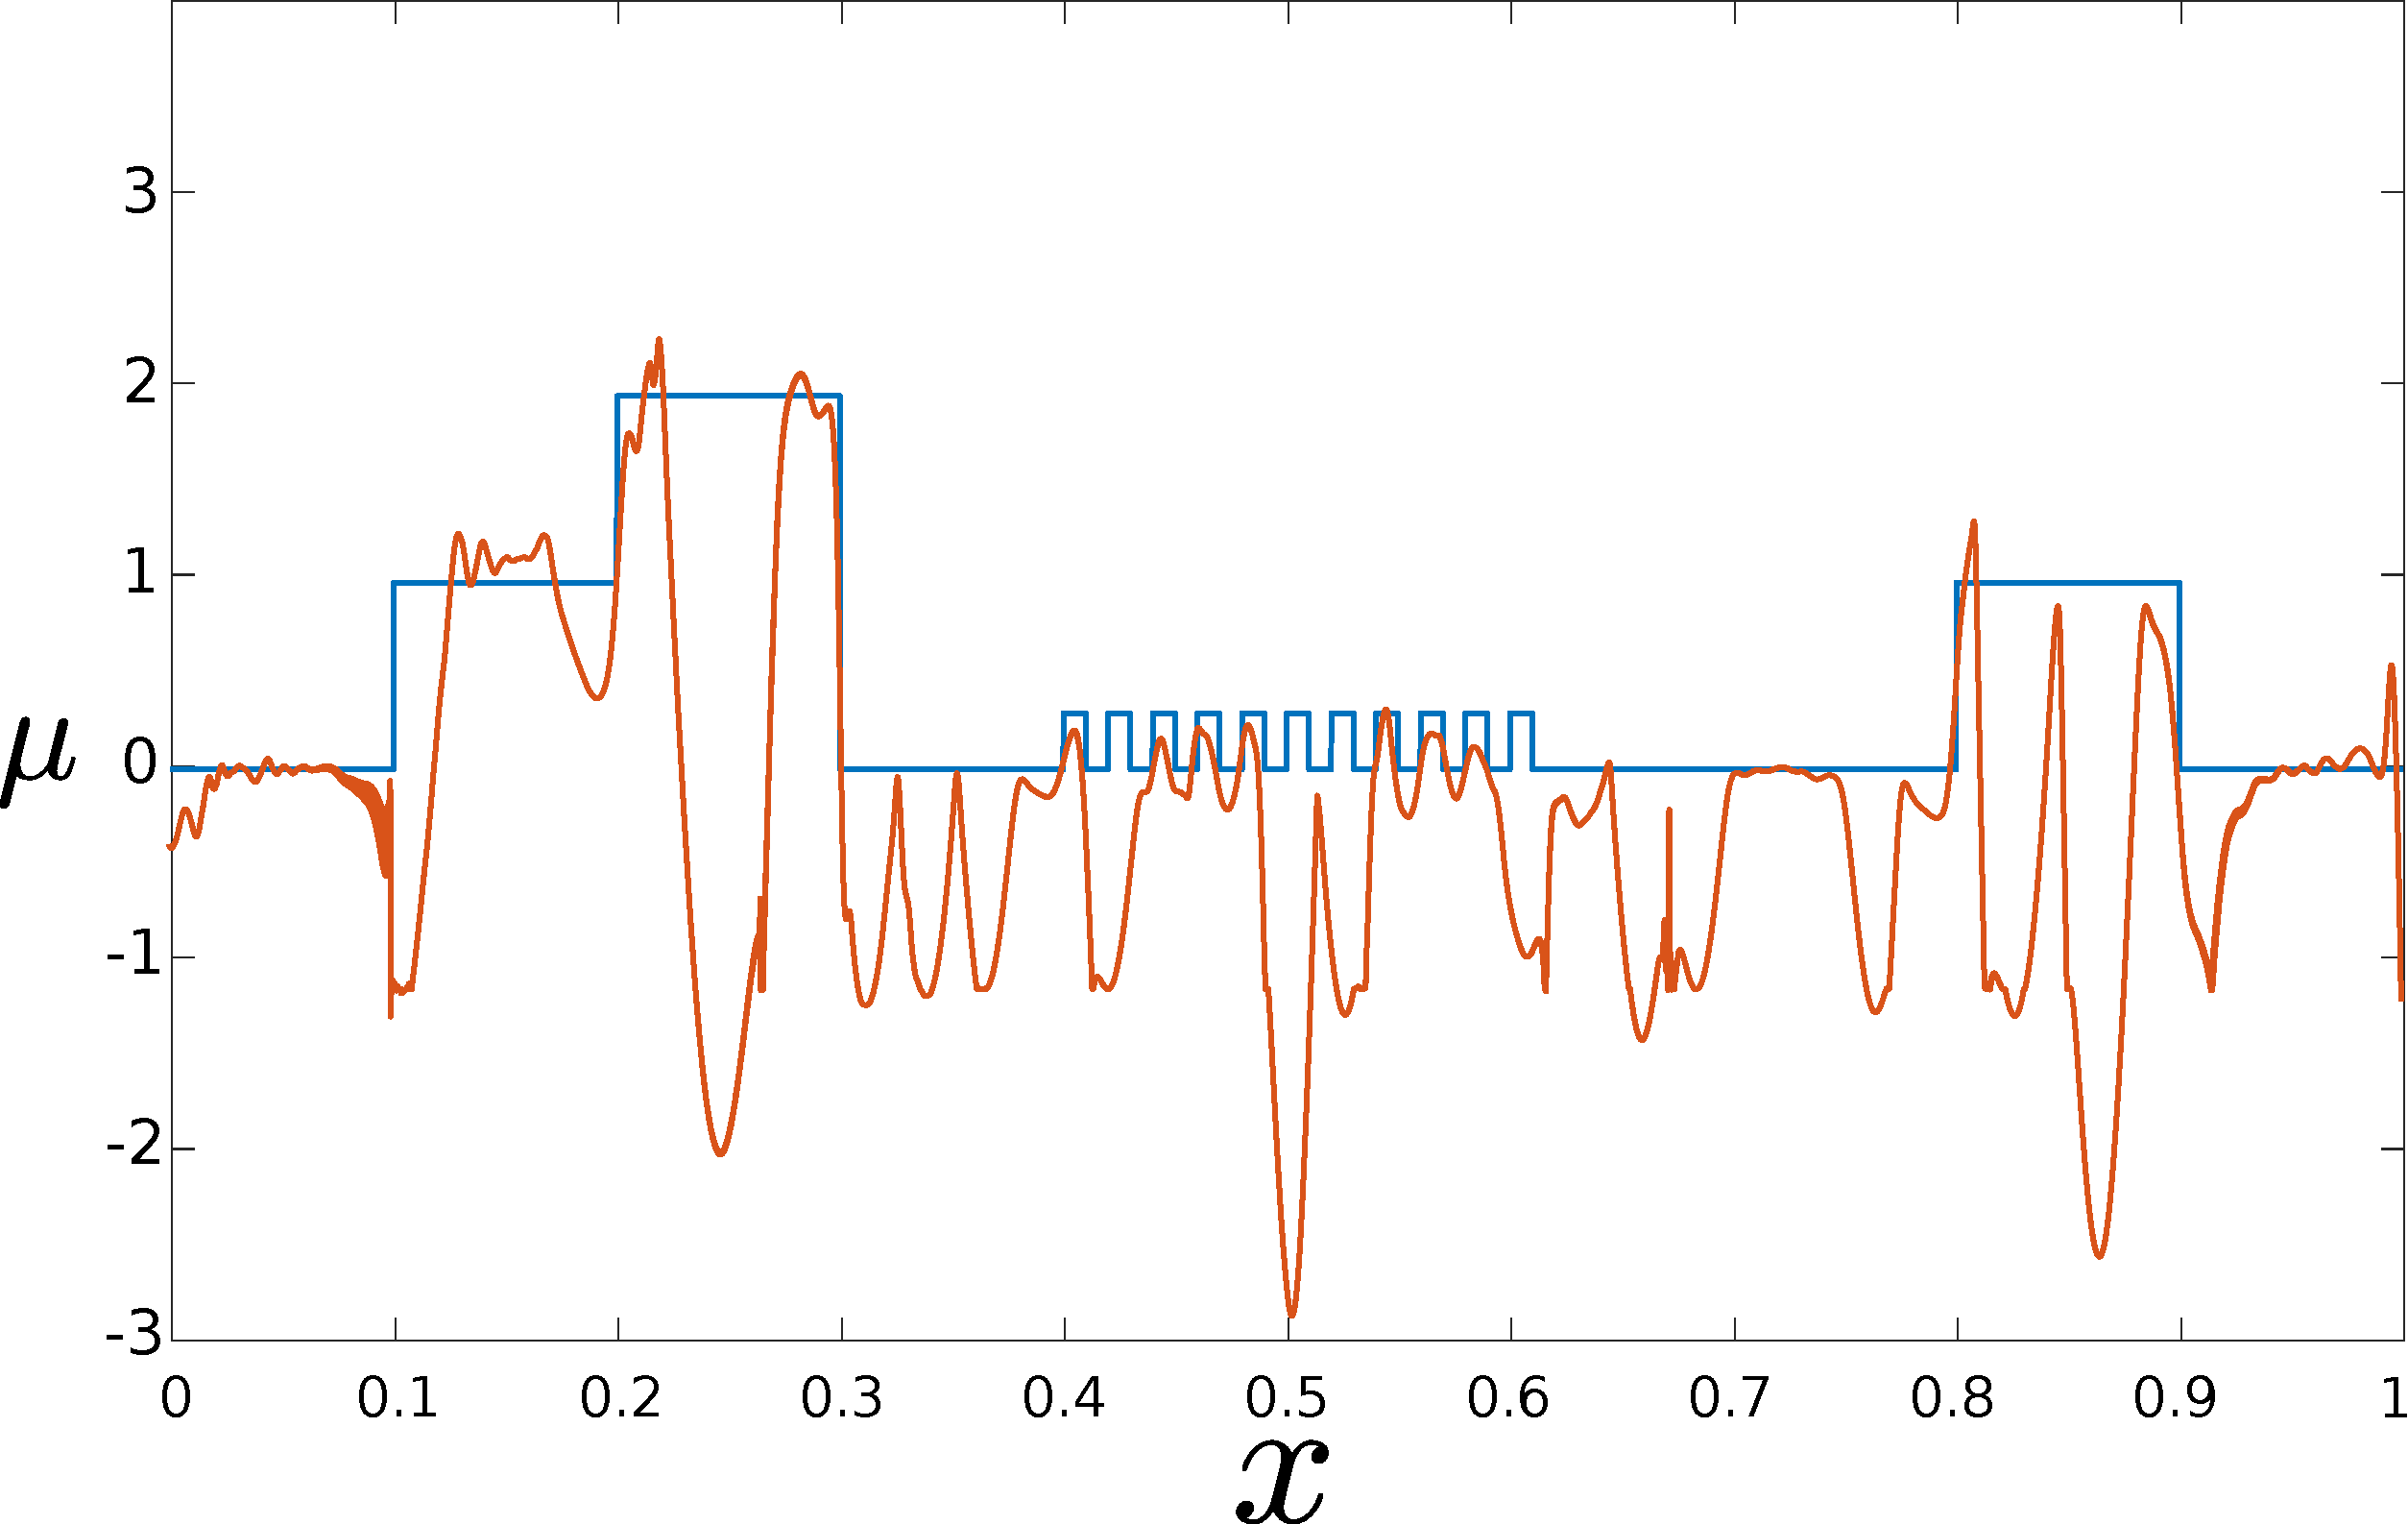
\includegraphics[width=0.8\textwidth]{Images/muCorrupted.pdf}
\centering
\caption{Original and reconstructed shear parameter $\mu$.}
\end{figure}
\end{frame}

\begin{frame}
 \begin{figure}
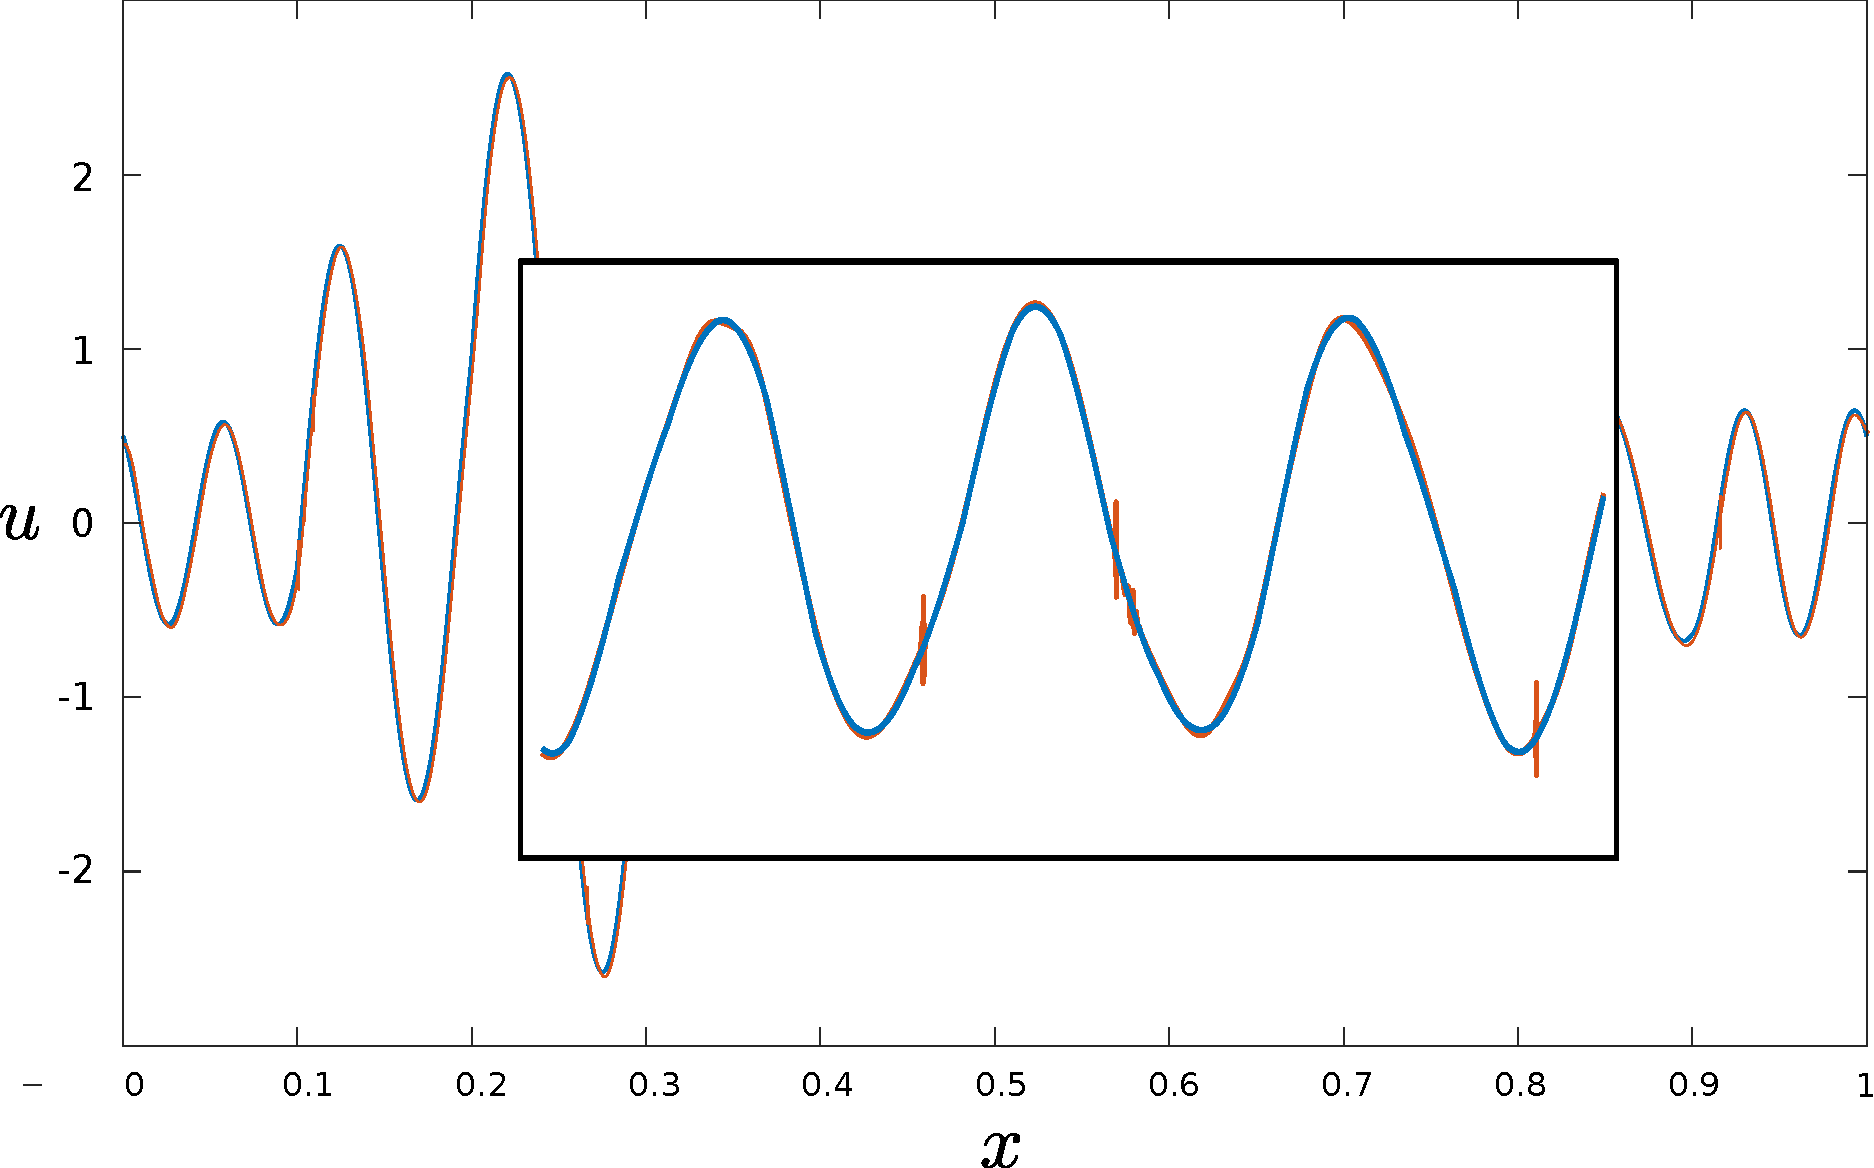
\includegraphics[width=0.8\textwidth]{Images/littleSpikesClose.pdf}
\caption{First derivative of original and denoised displacement $u$. Close-up reveals noise residuals on a fine scale.}
\centering\end{figure}
\end{frame}

\begin{frame}
 \begin{figure}
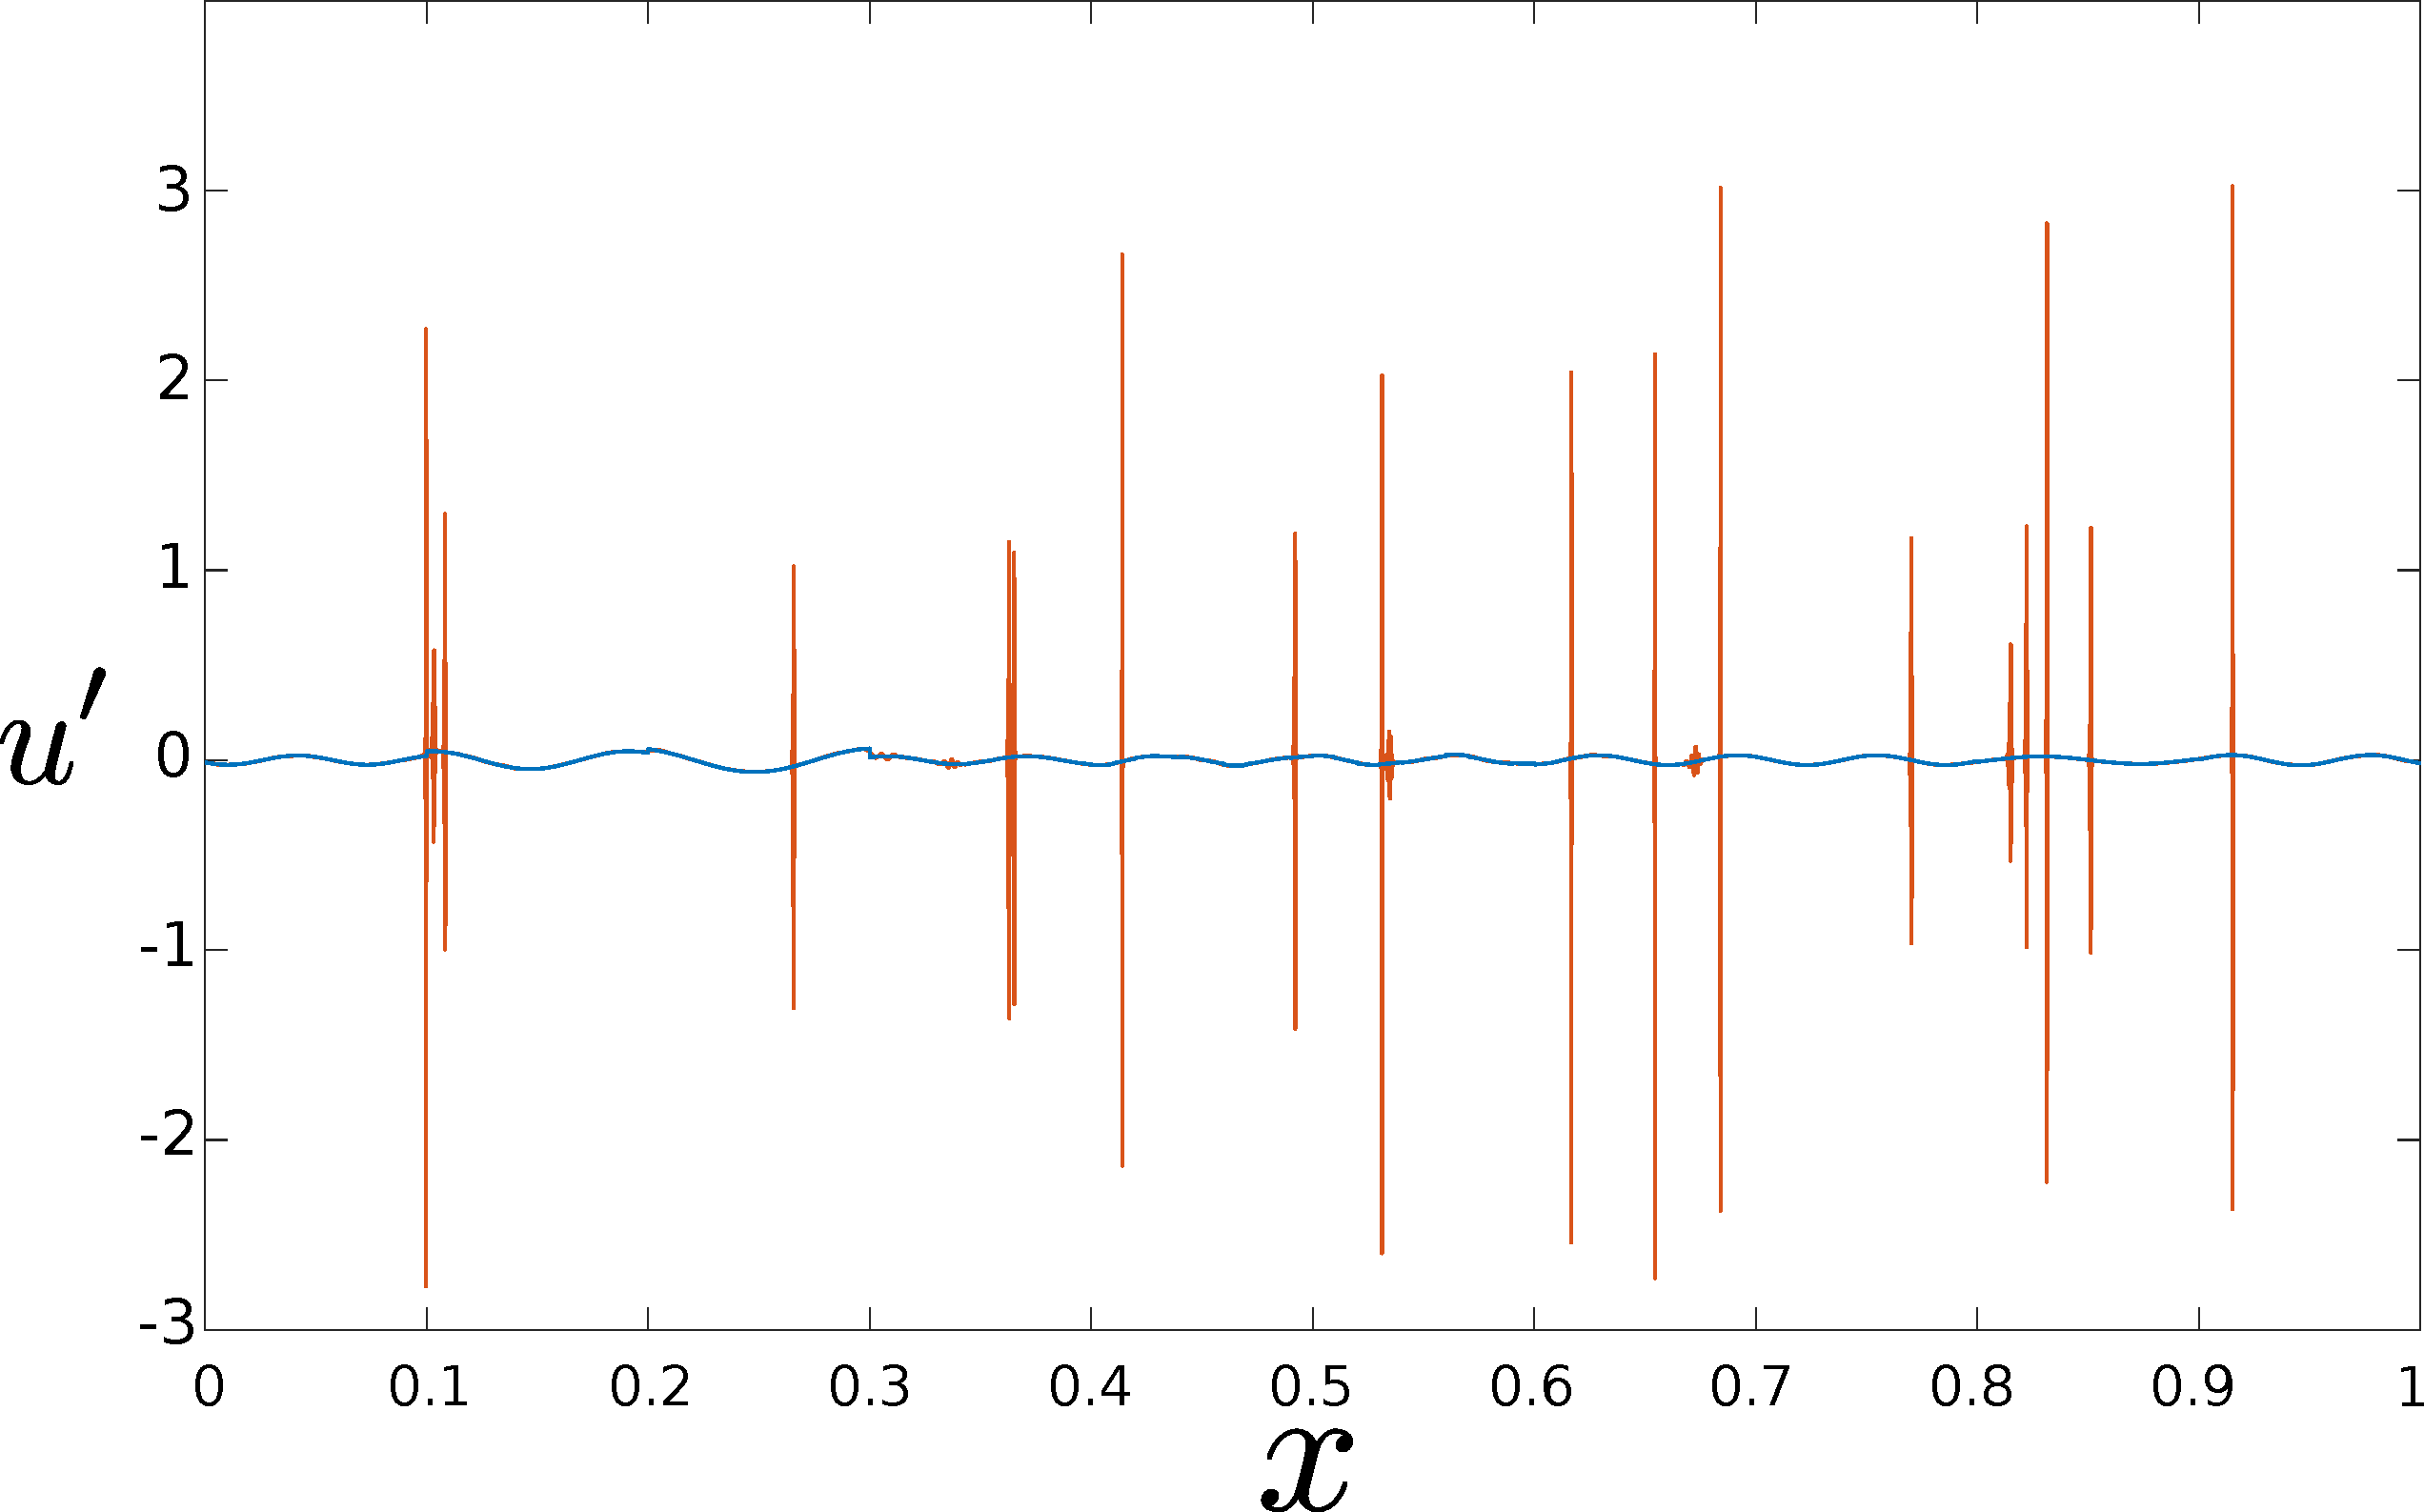
\includegraphics[width=0.8\textwidth]{Images/derivative.pdf}
\caption{First derivative of original and denoised displacement $u$. Fine scale noise dominates the first (and subsequent) derivatives.}
\centering\end{figure}
\end{frame}


\section{First Experiments}


\begin{frame}		\frametitle{Our plan of work}

\begin{itemize}
 \item Do simuations in 1d: wavelets
 \item Do simulations in 2d: wavelets, shearlets
 \item 
\end{itemize}

\begin{itemize}
 \item Problem: Need to reconstruct the derivatives
 \item slight noise can lead to totally wrong derivatives --> inversion is useless
 \item MRI measurement in 3 spatial directions and 8 time steps --> 
\end{itemize}

\end{frame}

\section{What comes next}


\begin{frame}		\frametitle{What would be nice results}

\begin{itemize}
 \item Have better resolution of the stiffness map
 \item Have clinically useful values, at the moment to varying
 \item Have shorter acquisition times per pixel
\end{itemize}

\begin{itemize}
 \item Problem: Need to reconstruct the derivatives
 \item slight noise can lead to totally wrong derivatives --> inversion is useless
 \item MRI measurement in 3 spatial directions and 8 time steps --> 
\end{itemize}

\end{frame}





 

\end{document}
